\documentclass[12pt]{article}
\usepackage[a4paper, margin=.30in]{geometry}
\usepackage{graphicx ,
            wrapfig,
            xcolor, 
            enumerate,
            amsmath,fontenc, mhchem,tikz, pgfplots
            }

\newcommand\headerMe[2]{\noindent{}#1\hfill#2}
\renewcommand{\thesection}{\Roman{section}}

\author{Zakaria HAOUZAN}
\date{\today}

\begin{document}
% headers --------------
\headerMe{Matière : Physique-Chimie}{Professeur : Zakaria HAOUZAN}\\
\headerMe{Unité : Transformations lentes et rapides\\ d'un système chimique }{Établissement : Lycée SKHOR qualifiant}\\
\headerMe{Niveau : 2BAC-SM-X}{Heure : 7H}\\


% ------Content ________
\begin{center}
	\Large{Leçon $N^{\circ} 2.2 $: \color{red} Suivi temporel d’une transformation - Vitesse de réaction }
\end{center}

\section{Techniques de suivi temporel d'une transformation :}

Pour suivre temporellement l'évolution d'une transformation chimique on doit connaître sa composition à chaque instant.
Il existe plusieurs méthodes qui permettent de suivre l'évolution d'une transformation chimique :
\\- Le dosage.
- La conductimétrie.
- La mesure de la pression.
- La pH-métrie.

\begin{wrapfigure}[1]{r}{0.3\textwidth}
	\vspace{-3cm}
	\includegraphics[width=0.27\textwidth]{./img/STidureavecperoxo.png}
\end{wrapfigure}



\section{suivi temporel d'une transformation :  }
\subsection{Activité 1 : Suivi par dosage }
\subsubsection{Expérience : }
Dans un bécher, verser 50 mL d'une solution incolore de peroxodisulfate de potassium,
$(2K^+_{(aq)} + {S_2O_8^{2-}}_{(aq)})$, à $0,10 mol.L^{-1}$ puis 50 mL d'une solution, incolore elle aussi, d'iodure de potassium, $(K^+_{(aq)} +I^-_{(aq)})$.
à $0.50 mol.L^-$

L'apparition progressive de la coloration jaune, caractéristique des molécules ${I_2}_{(aq)}$, montre que ces molécules sont formées par une réaction lente entre les ions peroxodisulfate ${S_2O_8}^{2-}$ et les ions iodure$I^-$.

\begin{enumerate}
	\item Écrivez l'équation de la réaction. sachant que $SO_4^{2-}/{S_2O_8^{2-}}_{(aq)}$
	\item Calculez les quantités de matière initiales des réactifs et tracez le tableau d’avancement.
	\item On recueille après chaque trois minutes $10cm^3$ du mélange réactionnel et on la trempe dans l'eau froide pour arrêter la réaction,Puis on dose le diiode $I_2$ formé par une solution de thiosulfate de sodium $(2Na^+ + {S_2O_3}^{2-})$  de concentration $Cr= 0,02mol/L$.

	      \begin{enumerate}
		      \item  Écrivez l'équation de la réaction de dosage, sachant que $S_4O_6^{2-}/{S_2O_3}^{2-} $
		      \item Déterminez l'expression de la quantité de matière de diiode à l'équivalence.
		      \item Complétez le tableau suivant :
		            \begin{center}
			            \begin{tabular}{|c|c|c|c|c|c|c|c|c|c|c|c|}
				            \hline
				            t(s)                & 0 & 3  & 6   & 9   & 12  & 16  & 20  & 30  & 40  & 50  & 60  \\\hline
				            V($S_2O_3^{2-} ml$) & 0 & 50 & 100 & 140 & 170 & 210 & 230 & 280 & 310 & 320 & 330 \\\hline
				            n($I_2 mmol$)       & 0 &    &     &     &     &     &     &     &     &     &     \\\hline
			            \end{tabular}
		            \end{center}
		      \item Tracez la courbe représentant la quantité de $I_2$ formé en fonction du temps.
		      \item Conclure
	      \end{enumerate}

\end{enumerate}

\subsubsection{Exploitation :}
\begin{itemize}
	\item Les ions peroxodisulfate $S_2O_8^{2-}$ oxydent les ions iodure $I^-$ selon une réaction d'équation:

	      $2I^-_{(ag)} + {S_2O_8^{2-}}_{(aq)} = {I_2}_{(aq)} + 2{SO_4^{2-}}_{(aq)}$ (1)

	\item Cette réaction nétant pas trop rapide, elle peut être suivie en dosant le
	      diode formé.

	\item On peut également utiliser la spectrophotométrie puisque la réaction met en jeu une seule espèce colorée, le diiode.

	\item Les ions iodures $I^-$ sont lentement oxydés par les ions peroxodisulfate ce qui entraine la formation progressive du diiode $I_2$.
	      Pour savoir la quantité du diiode qui s'est formée à un instant donné on réalise le dosage.


	      %\begin{figure}[h!]
	      \begin{center}
		      \includegraphics[width=0.2\textwidth]{./img/STlatrempe.png}
		      \includegraphics[width=0.2\textwidth]{./img/STmotageDosage.png}
	      \end{center}

	      %\end{figure}
	\item Les deux couples mis en jeux durant le dosage sont :$I_2/I^-$ ET $S_4O_6^{2-}/S_2O_3^{2-}$.
	\item Equation de la réaction du dosage: \ce{2S_2O_3^{2-} + I_2 -> S_4O_6^{2-} + 2I^-}
	      c'est une réaction rapide
	\item à l'équivalence : $\frac{n(S_2O_3^{2-})}{2} = \frac{n(I_2)}{1}$

	\item Soit vr le volume de la solution de thiosulfate de sodium ajoutée à l'équivalence. $n(I_2) = \frac{C_r.V_r}{2}$

	\item Tableau des mesures:

	      \begin{center}
		      \begin{tabular}{|c|c|c|c|c|c|c|c|c|c|c|c|}
			      \hline
			      t(s)          & 0 & 3   & 6   & 9   & 12  & 16  & 20  & 30  & 40  & 50  & 60  \\\hline
			      n($I_2 mmol$) & 0 & 0.5 & 1.0 & 1.4 & 1.7 & 2.1 & 2.3 & 2.8 & 3.1 & 3.2 & 3.3 \\\hline
		      \end{tabular}
	      \end{center}



\begin{figure}[htbp] % htbp for better positioning options
    \centering
    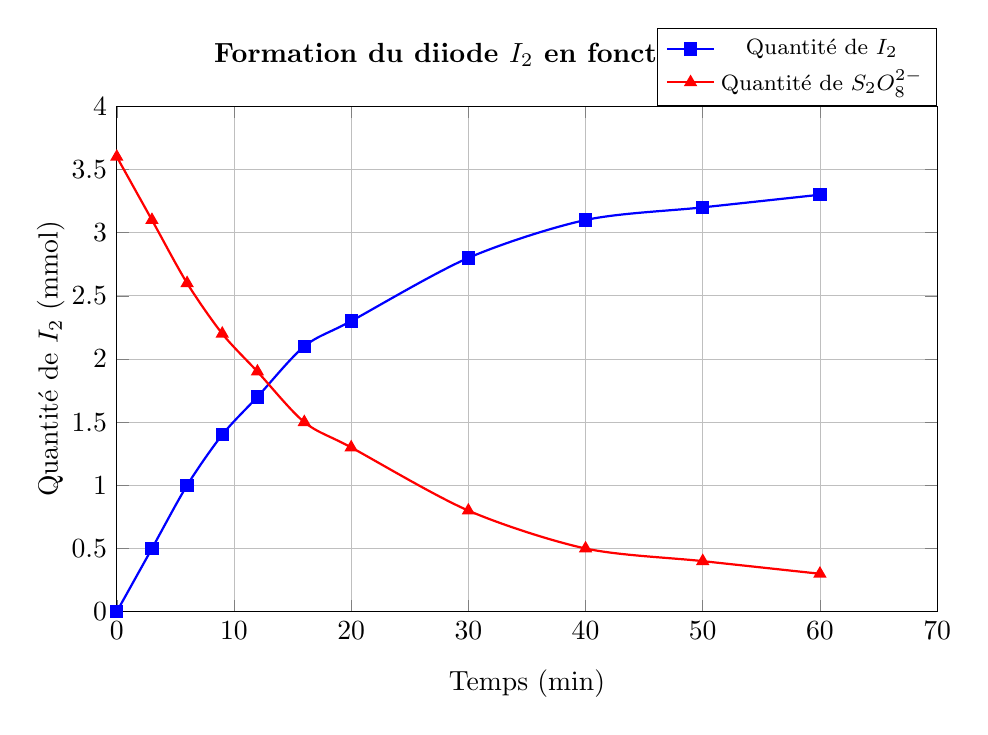
\begin{tikzpicture}
        \begin{axis}[
            xlabel={Temps (min)},
            ylabel={Quantité de \(I_2\) (mmol)},
            xmin=0, xmax=70,
            ymin=0, ymax=4,
            xtick={0,10,20,30,40,50,60,70}, % Adjusting x-ticks for clarity
            ytick={0,0.5,1,1.5,2,2.5,3,3.5,4}, % Adjusting y-ticks for clarity
            grid=both,
            major grid style={line width=0.3pt, draw=gray!50}, % Slightly thicker major grid lines
            minor grid style={line width=0.1pt, draw=gray!30},
            width=12cm, height=8cm, % Making the figure slightly larger
            legend pos=north west,
            legend style={font=\footnotesize, at={(1,1)}, anchor=south east}, % Adjust legend positioning
            title={Formation du diiode \(I_2\) en fonction du temps}, % Adding a title for context
            title style={yshift=1ex, font=\normalsize\bfseries}, % Styling title
            ylabel style={yshift=-1ex}, % Positioning y-label slightly lower
            xlabel style={yshift=-1ex}, % Positioning x-label slightly lower
        ]
        \addplot[
            color=blue,
            mark=square*,
            thick,
            smooth, % Smoothing the line for better visualization
        ]
        coordinates {
            (0,0) (3,0.5) (6,1.0) (9,1.4) (12,1.7) (16,2.1) (20,2.3) (30,2.8) (40,3.1) (50,3.2) (60,3.3)
        };
        \addlegendentry{Quantité de \(I_2\)}

   % Second curve for the new data
        \addplot[
            color=red,
            mark=triangle*,
            thick,
            smooth, % Smoothing the line for better visualization
        ]
        coordinates {
            (0,3.6) (3,3.1) (6,2.6) (9,2.2) (12,1.9) (16,1.5) (20,1.3) (30,0.8) (40,0.5) (50,0.4) (60,0.3)
        };
          \addlegendentry{Quantité de \(S_2O_8^{2-}\)}

        \end{axis}
    \end{tikzpicture}
    \caption{Variation de la quantité de diiode \(I_2\) en fonction du temps.}
\end{figure}



	\item Tableau d'avancement

	      \begin{tabular}{|c|c|c|c|c|c|}
		      \hline
		      \multicolumn{2}{|c|}{Equation de la réaction} & \multicolumn{4}{c|}{${ S_2O_8^{2-} + 2I^- \rightarrow 2S_2O_4^{2-} + I_2}$}                                                                                                        \\\hline
		      états                                         & avancement                                                                  & \multicolumn{4}{|c|}{quantité de Matière en mol}                                                     \\\hline
		      Etat initial                                  & 0                                                                           & $ C_2.V_2$                                       & $ C_1.V_1$             & $ 0$       & $ 0$        \\\hline
		      Etat de transformation                        & $x$                                                                         & $ C_2.V_2 - x$                                   & $ C_1.V_1 -  2x$       & $ 2x$      & $ x$        \\\hline
		      Etat final                                    & $x_{max}$                                                                   & $  C_2.V_2 - x_{max}$                            & $  C_1.V_1 - 2x_{max}$ & $2x_{max}$ & $  x_{max}$ \\\hline
		      % \cline{2-4}\
	      \end{tabular}

	\item D'après le tableau d'avancement, la quantité du diiode formée à un instant t est égale à x.${n(I_2)}_t$=$x$. Donc le dosage nous permet de suivre l'évolution de la formation du diiode en fonction du temps et de déterminer l'avancement.
	\item Le tracé montre que la quantité du diiode formée augmente en fonction du temps.
	      On peut déterminer les quantités de matières des autres constituants du mélange réactionnel en fonction du temps.

	\item Exemple : $n(S_2O_8^{2-}) = C_2.V_2 - x$ avec $C_2 = 0.036mol/L$  et $V_2 = 100ml$ donc $n(S_2O_8^{2-}) = 3.6 - x $

	      \begin{center}
		      \begin{tabular}{|c|c|c|c|c|c|c|c|c|c|c|c|}
			      \hline
			      t(s)                  & 0   & 3   & 6   & 9   & 12  & 16  & 20  & 30  & 40  & 50  & 60  \\\hline
			      $x (mmol$)            & 0   & 0.5 & 1.0 & 1.4 & 1.7 & 2.1 & 2.3 & 2.8 & 3.1 & 3.2 & 3.3 \\\hline
			      n($S_2O_8^{2-} mmol$) & 3.6 & 3.1 & 2.6 & 2.2 & 1.9 & 1.5 & 1.3 & 0.8 & 0.5 & 0.4 & 0.3 \\\hline
		      \end{tabular}
	      \end{center}

	      Le tracé décroissant montre que la quantité de $S_2O_8^{2-}$ diminue en fonction du temps.

\end{itemize}


\section{Vitesse de la réaction - Temps demi réaction :  }

\subsection{Vitesse de la réaction}
\subsubsection{Définition:}
La vitesse volumique d’une réaction correspond à la quantité de matière formée ou disparue par unité de temps et de volume.
Elle est liée à la variation de l’avancement x de la réaction en fonction du temps par la relation suivante:
$$v = \frac{1}{V}.\frac{dx}{dt}$$

$v : $ vitesse volumique de la réaction en ($mol/m^3.s$).

$\frac{dx}{dt}$ : dérivée de l'avancement en (mol/s)

$V$ : volume totale de la solution.

En général, la vitesse de la réaction diminue lors de l'évolution d'une transformation chimique.

\begin{wrapfigure}[2]{r}{0.3\textwidth}
	\vspace{-1.5cm}
	\includegraphics[width=0.3\textwidth]{./img/STvitesse.png}
\end{wrapfigure}


\section*{Détermination graphique de la vitesse de la réaction:++}
On détermine la vitesse de la réaction à un instant t donné, en traçant la droite tangente à la courbe $x=f(t)$ à cet instant puis on détermine le coefficient directeur de cette droite et on le divise par le volume V de la solution.

en choisissant deux points A et B appartenant à cette droite de la manière suivante : $\alpha$
Le coefficient directeur
$$\alpha = \frac{\Delta{x}}{\Delta{t}} = \frac{x_B - x_A}{t_B - t_A} = \frac{dx}{dt}$$
$$v = \frac{1}{V}.\frac{dx}{dt} = \frac{1}{V}.\frac{x_B - x_A}{t_B - t_A}$$

\begin{wrapfigure}[1]{r}{0.3\textwidth}
	\vspace{-3cm}
	\includegraphics[width=0.3\textwidth]{./img/STdemi_rection.png}
\end{wrapfigure}

\subsubsection{Temps de demi-réaction}
On appelle temps de demi-réaction t1/2 le temps nécessaire pour que l'avancement de la réaction soit égal à la moitié de sa valeur finale. $x(t_{1/2}) = \frac{x_f}{2}$

Si la réaction est totale $x_f=x_{max}$ dans ce cas: $x(t_{1/2}) = \frac{x_{max}}{2}$




\newpage
\begin{wrapfigure}[2]{r}{0.3\textwidth}
  \vspace{-3cm}
	\includegraphics[width=0.3\textwidth]{./img/STpressionavec_balon.png}
\end{wrapfigure}



\subsection{Activité 2 : Suivi par mesure de pression }
\subsubsection{Expérience: }
On introduit un ruban de magnésium de masse $m=0,02g$ dans ballon contenant un volume $V=50cm3$
d'une solution d'acide chlorhydrique ($H^+_{(aq)} + Cl^-_{(aq)}$) de concentration $C=0,5mol/L$ puis on mesure la pression du gaz résultant par un manomètre.

\vspace{0.2cm}

On constate que le magnésium réagit avec l'acide chlorhydrique avec dégagement d'hydrogène et cette réaction dure quelques
minutes jusqu'à la disparition totale du ruban de magnésium.

\begin{enumerate}
  \item Ecrire l'équation de la réaction sachant que les deux couples mis en jeux sont : $H^+/H_2$ et $Mg^{2+}/Mg$
  \item Calculez la quantité de matière initiale de magnésium et tracez le tableau d’avancement.
  \item Montrez que l'avancement de la réaction s'écrit : \(x = \frac{P_t-P_{atm}}{P_{x_{max}}-P_{atm}}.x_{max}\)
  \item La pression dans le ballon est mesurée toutes les 30 secondes. Complétez le tableau suivant:
	      \begin{center}
		      \begin{tabular}{|c|c|c|c|c|c|c|c|c|c|c|c|c|}
			      \hline
			      t(s)      & 0    & 30   & 60   & 90   & 120  & 150  & 180  & 210  & 240  & 270  & 300  & 330  \\\hline
			      P($hPa$)  & 1013 & 1025 & 1036 & 1048 & 1060 & 1068 & 1097 & 1081 & 1087 & 1091 & 1093 & 1093 \\\hline
			      x($mmol$) &     &  &  &  &  &  &  &   &  &   &  & 0.82 \\\hline
		      \end{tabular}
	      \end{center}

		      \item Tracez la courbe représentant l'avancement en fonction du temps.
          \item Déterminez la vitesse de réaction à t = 30 s et à t = 120 s.
          \item Estimez le temps de demi-réaction.
\end{enumerate}


%\begin{wrapfigure}[2]{r}{0.2\textwidth}
%\end{wrapfigure}


\subsubsection{Exploitation:}
\begin{itemize}
  \item  l'Equation de la reaction:  \ce{$Mg_{(s)} + 2H^+$ -> $Mg^{2+}_{(aq)} + {H_2}_{(g)}$}
	\item La quantité de matière initiale du magnésium : $n_0(Mg) = \frac{m(Mg)}{M(Mg)} = \frac{0.02g}{24.3g/mol} = 0.82mmol$
	\item La quantité de matière initiale des ions $H^+$: ${n_0(H^+)}_{(aq)} = c.v = 0.5mol/L . 50.10^{-3}mol = 25mmol$
	\item Tableau d'avancement

	      \begin{tabular}{|c|c|c|c|c|c|}
		      \hline
		      \multicolumn{2}{|c|}{Equation de la réaction} & \multicolumn{4}{c|}{$ Mg + 2H^+ \rightarrow  Mg^{2+} + H_2$}                                                                                               \\\hline
		      états                                         & avancement                                                   & \multicolumn{4}{|c|}{quantité de Matière en mol}                                            \\\hline
		      Etat initial                                  & 0                                                            & $ 0.82$                                          & $ 25$          & $ 0$      & $ 0$        \\\hline
		      Etat de transformation                        & $x$                                                          & $ 0.82- x$                                       & $ 25-2x$       & $ x$      & $ x$        \\\hline
		      Etat final                                    & $x_{max}$                                                    & $ 0.82-x_{max}$                                  & $25- 2x_{max}$ & $x_{max}$ & $  x_{max}$ \\\hline
		      % \cline{2-4}\
	      \end{tabular}

	\item Or la réaction continue jusqu'à la disparition totale du ruban de magnésium, Mg est le réactif limitant. $x_{max} = 0.82mmol$
	\item D'après le tableau d'avancement à un instant t(état de transformation) $n(H_2)$ et à état final $n(H_2)$=$x_{max}$

	\item la pression est liée à la quantité de matière du l'hydrogène gazeux résultant de la réaction par la relation $${P}_{(H_2)}.V = n_{(H_2)}.R.T \hspace{1cm} P_{(H_2)} =\frac{n_{(H_2)}.R.T}{V} \hspace{2cm}  (1)$$

	\item À l'instant t=o la pression dans le ballon est égale à la pression atmosphérique.
	\item À un instant t la pression dans le ballon (indiquée par le manomètre) est : $P = P_{atm} + P_{(H_2)}$ donc $P_{(H_2)}= P-P_{atm}$

	\item Donc à un instant t la relation (1) devient : $ P_{(H_2)}= P_t-P_{atm} = \frac{x.R.T}{V}$ (1')

	\item Et à la fin de la réaction elle devient : $ P_{(H_2)}= P_{max}-P_{atm} = \frac{x_{x_{max}}.R.T}{V}$ (1")

	      En divisant (1') par (1") on obtient ($x = n(H_2)$): $$x = \frac{P_t-P_{atm}}{P_{x_{max}}-P_{atm}}$$

	\item Tableau des mesures:($P_{atm}=1013hPa$ et $P_{max}=1093hPa$)

	      \begin{center}
		      \begin{tabular}{|c|c|c|c|c|c|c|c|c|c|c|c|c|}
			      \hline
			      t(s)      & 0    & 30   & 60   & 90   & 120  & 150  & 180  & 210  & 240  & 270  & 300  & 330  \\\hline
			      P($hPa$)  & 1013 & 1025 & 1036 & 1048 & 1060 & 1068 & 1097 & 1081 & 1087 & 1091 & 1093 & 1093 \\\hline
			      x($mmol$) & 0    & 0.12 & 0.24 & 0.36 & 0.48 & 0.56 & 0.68 & 0.7  & 0.76 & 0.8  & 0.82 & 0.82 \\\hline
		      \end{tabular}
	      \end{center}



\begin{figure}[htbp]
    \centering
    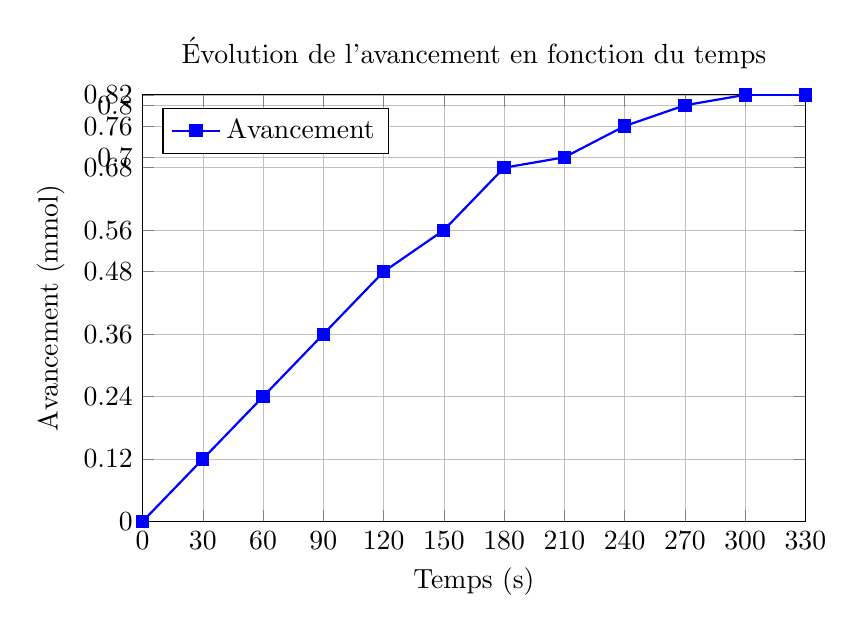
\begin{tikzpicture}
        \begin{axis}[
            xlabel={Temps (s)},
            ylabel={Avancement (mmol)},
            xmin=0, xmax=330,
            ymin=0, ymax=0.82,
            xtick={0,30,60,90,120,150,180,210,240,270,300,330},
            ytick={0,0.12,0.24,0.36,0.48,0.56,0.68,0.7,0.76,0.8,0.82},
            grid=both,
            major grid style={line width=.2pt,draw=gray!50},
            minor grid style={line width=.1pt,draw=gray!30},
            width=10cm, height=7cm,
            legend pos=north west,
            title={Évolution de l'avancement en fonction du temps}
        ]
        \addplot[
            color=blue,
            mark=square*,
            thick
        ]
        coordinates {
            (0,0) (30,0.12) (60,0.24) (90,0.36) (120,0.48) 
            (150,0.56) (180,0.68) (210,0.7) (240,0.76) 
            (270,0.8) (300,0.82) (330,0.82)
        };
        \addlegendentry{Avancement}
        \end{axis}
    \end{tikzpicture}
    \caption{Courbe de l'avancement en fonction du temps.}
    \label{fig:avancement_time}
\end{figure}

\end{itemize}






\subsection{Activité 3 : Suivi par conductimétrie }
\subsection{Expérience : }
On introduit dans un bécher un peu d'eau et d'éthanol et on ajoute au mélange $1cm^3$ de 2-chloro 2-méthyle propane de formule semi-développée : $(CH_3)-C-Cl$ qu’on notera simplement $R-Cl$.

L'éthanol est un solvant dans lequel $R-Cl$ se dissout très facilement et sans réagir avec l'éthanol.

\begin{enumerate}
  \item Écrivez l'équation de la réaction.
  \item Calculez la quantité de matière initiale de R-Cl (masse volumique = 0,85 g/cm³, M = 92,5 g/mol).
  \item Montrez que l'avancement de la réaction s'écrit : \(\sigma_t = \frac{\sigma_t}{\sigma_{max}}.x_{max}\)
  \item La conductivité de la solution est mesurée toutes les 2 minutes. Complétez le tableau suivant:

    \begin{center}
		      \begin{tabular}{|c|c|c|c|c|c|c|c|c|c|c|c|c|}
			      \hline
			      t(s)          & 0 & 200   & 400   & 600   & 800   & 1000  & 1200  & 1400  & 1600  & 1800  & 2000  & 2200  \\\hline
			      $\sigma(S/m)$ & 0 & 0.489 & 0.977 & 1.270 & 1.466 & 1.661 & 1.759 & 1.856 & 1.905 & 1.955 & 1.955 & 1.955 \\\hline
			      x($mmol$)     & & & & & & & & & & & & \\\hline
		      \end{tabular}
	      \end{center}


  \item Tracez la courbe représentant l'avancement de la réaction en fonction du temps.
  \item Déterminez la vitesse de réaction à t = 2 min et à t = 8 min.
  \item Estimez le temps de demi-réaction.
\end{enumerate}


\subsubsection{Exploitation: }
\begin{itemize}
	\item la quantité de matière initiale avec $\rho(R-Cl) = 0.85g/cm^3$ et $M(R-Cl) = 92.5 g/mol$

	      $n_0 = \frac{m}{M} =\frac{\rho.V}{M} = \frac{0.85g/cm^3 . 1cm^3}{92.5 g/mol} \approx 9.2 10^{-3} mol$
	\item Tableau d'avancement

	      \begin{tabular}{|c|c|c|c|c|c|c|}
		      \hline
		      \multicolumn{2}{|c|}{Equation de la réaction} & \multicolumn{5}{c|}{$ R-Cl + H_2O \rightarrow  R-OH + H^++ Cl^-$}                                                                                                        \\\hline
		      états                                         & avancement                                                        & \multicolumn{5}{|c|}{quantité de Matière en mol}                                                     \\\hline
		      Etat initial                                  & 0                                                                 & $ n_0$                                           & par excès & $ 0$      & $ 0$        & 0           \\\hline
		      Etat de transformation                        & $x$                                                               & $ n_0- x$                                        & par excès & $ x$      & $ x$        & x           \\\hline
		      Etat final                                    & $x_{max}$                                                         & $ n_0-x_{max}$                                   & par excès & $x_{max}$ & $  x_{max}$ & $  x_{max}$ \\\hline
		      % \cline{2-4}\
	      \end{tabular}

	      H2O étant utilisée en excès , RCl est le réactif limitant . $x_{max} = n_0$

	\item La conductivité de la solution est : $$\sigma = \lambda_{H^+}.[H^+] + \lambda_{Cl^-}.[Cl^-]$$

	      On a : $\sigma = (\lambda_{H^+} + \lambda_{Cl^-}).\frac{x}{V}$ et $[H^+]= [Cl^-] =\frac{x}{V}$
	      Donc : $$\sigma_t = (\lambda_{H^+} + \lambda_{Cl^-}).\frac{x}{V} \hspace{1cm} (1) $$
	      $$\sigma_{max} = (\lambda_{H^+} + \lambda_{Cl^-}).\frac{x_{max}}{V} \hspace{1cm}  (2)$$

	\item En divisant (1) par (2) on obtient: $x = \frac{\sigma_t}{\sigma_{max}}. x_{max}$

	\item Tableau des mesures:($\sigma_{max}=1.955Sm^{-1}$ et $x=\frac{\sigma_t.9.210^{-3}}{1.955}$)

	      \begin{center}
		      \begin{tabular}{|c|c|c|c|c|c|c|c|c|c|c|c|c|}
			      \hline
			      t(s)          & 0 & 200   & 400   & 600   & 800   & 1000  & 1200  & 1400  & 1600  & 1800  & 2000  & 2200  \\\hline
			      $\sigma(S/m)$ & 0 & 0.489 & 0.977 & 1.270 & 1.466 & 1.661 & 1.759 & 1.856 & 1.905 & 1.955 & 1.955 & 1.955 \\\hline
			      x($mmol$)     & 0 & 2.3   & 4.6   & 5.98  & 6.9   & 7.82  & 8.32  & 8.64  & 8.96  & 9.20  & 9.20  & 9.20  \\\hline
		      \end{tabular}
	      \end{center}
\end{itemize}

\section*{La vitesse de la réaction et les facteurs cinétiques: }
Plus la température est élevée, plus les risques de collisions sont élevés et plus la réaction est rapide.
Plus les concentrations initiales de réactifs sont élevées, plus la probabilité de collisions est grande et donc plus la réaction est
rapide.
\section*{++bonus++}
Quand la température croît, le nombre des chocs intermoléculaires par unité de temps et de volume et leur efticacité augmentent.

C'est pourquoi la vitesse d'évolution d'un système chimique croît avec la température.

-Caractère aléatoire des chocs :
\begin{itemize}
	\item Les chocs ont lieu au hasard des déplacements des différentes entités: ils
	      sont aléatoires".

	\item Il arrive donc que des chocs efficaces se déroulent entre des molécules de
	      produits, provoquant leurs transformations en molécules de réactifs: la
	      réaction directe et la réaction inverse se déroulent alors simultanément dans
	      le système.

	\item La vitesse de la réaction inverse augmente avec la concentration de ses
	      réactifs, c'est-à-dire avec celle des produits de la réaction directe: lorsque la
	      vitesse de la réaction directe et celle de la réaction inverse sont égales, la
	      composition du système n'évolue plus.

\end{itemize}

\end{document}
%\begin{figure}[h!]
%\begin{center}
%\includegraphics[width=0.5\textwidth]{./img/TRLconcentration.png}
%\end{center}
%\vspace{-1cm}
%\end{figure}



%\begin{wrapfigure}[10]{r}{0.5\textwidth}
%    \includegraphics[width=0.5\textwidth]{./img/img00.png}
%\end{wrapfigure}


%\begin{center}
%\begin{tabular}{|c|c|c|}
%\hline
%Indicateur coloré & Couleur de l’espèce acide & Couleur de l’espèce base\\\hline
%BBT               & Jaune                     & Bleue\\\hline
%Hélianthine       &Rose                       & Jaune\\\hline
%Phénolphtaléine   & inclore                   & rose \\\hline
%\end{tabular}
%\end{center}


